\documentclass{article}
\usepackage{geometry}
\usepackage[cm]{fullpage}
\usepackage{amsmath, amsthm, graphicx, enumitem, amssymb, listings, verbatim, xcolor,scrextend,commath,multirow,pbox,dashrule,
bm
}

\usepackage[T1]{fontenc}
\usepackage{sansmath}

\newcommand{\percent}{$1\%$ }
\begin{document}

\setlength{\abovedisplayskip}{2.5pt}
\setlength{\belowdisplayskip}{2.5pt}

We sampled about \percent of the total comments, which took about 20 minutes (without training model) to generate all required csv files for the deliverable.
\begin{enumerate}
\item Time series plot (by day) of positive and negative sentiments.
\begin{figure*}[!ht]
\centering
\caption{Time series plot}
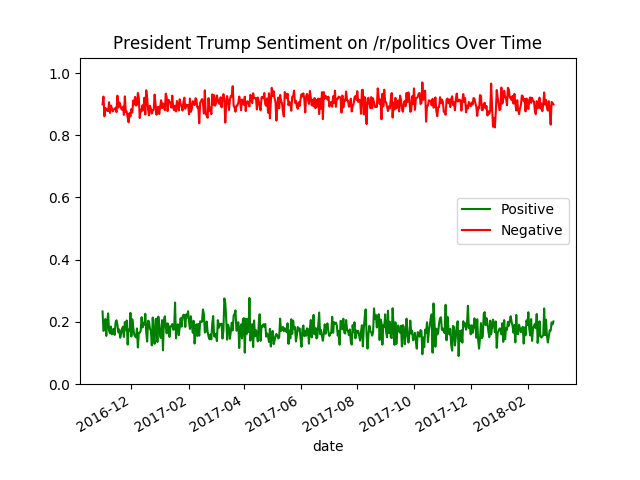
\includegraphics[width=0.6\textwidth]{part1.png}	
\end{figure*}

\item 2 maps of the United States: one for positive sentiment and one for negative sentiment. Color the states by the percentage.  \\
\textbf{Extra credit:} we have successfully added Alaska and Hawaii to the map.
\begin{figure*}[!ht]\centering
\caption{Map of positive sentiment}
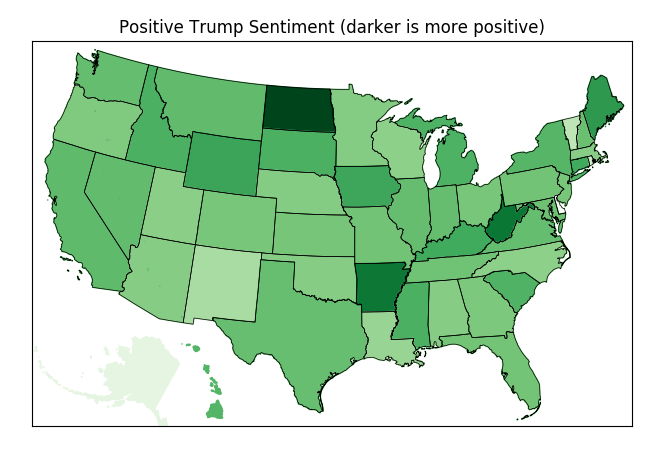
\includegraphics[width=0.6\textwidth]{posmap.png}	
\end{figure*}
\newpage
\begin{figure*}[!ht]\centering
\caption{Map of negative sentiment}
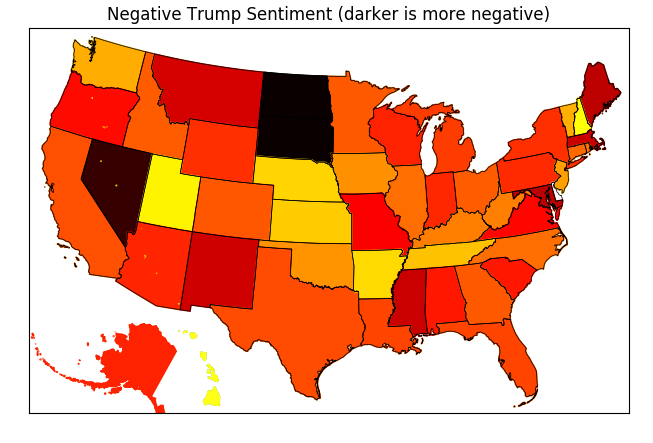
\includegraphics[width=0.6\textwidth]{negmap}	
\end{figure*}


\item Map of United States that computes Positive percentage $-$ Negative percentage
\begin{figure*}[!ht]
\centering
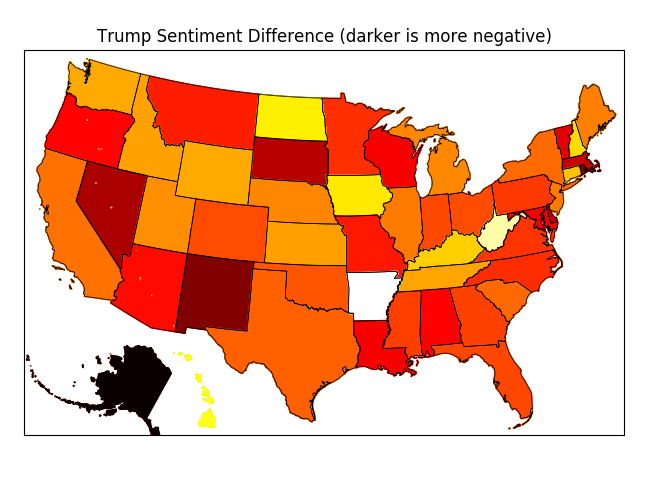
\includegraphics[width=.6\textwidth]{diffmap.png}	
\end{figure*}

\newpage
\item For the \percent of the data that we sampled, the list of ``most positive'' scores are:
\begin{figure*}[!ht]
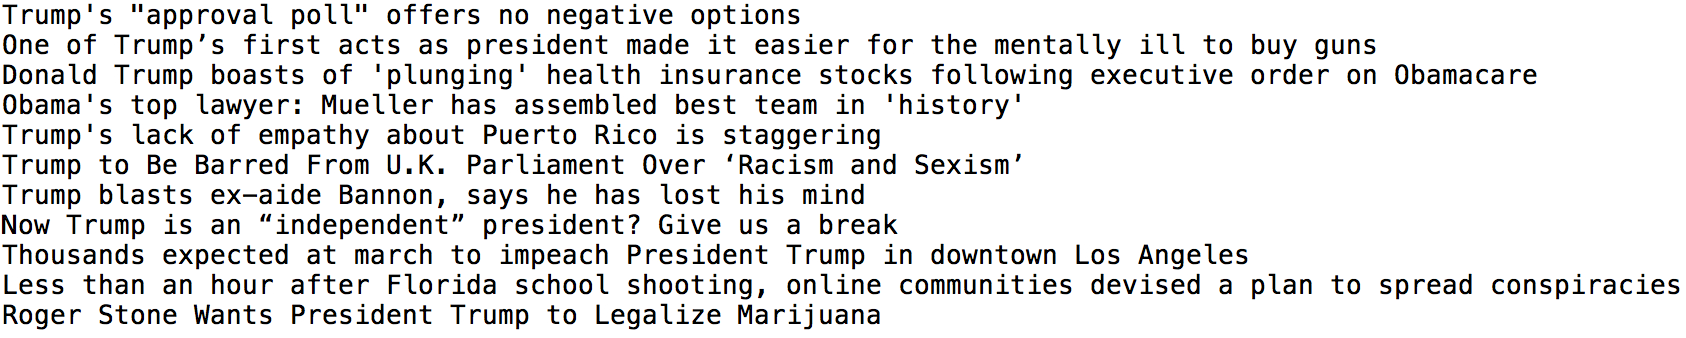
\includegraphics[width=.8\textwidth]{pos10.png}	
\end{figure*}

\indent The most negative stories are
\begin{figure*}[!ht]
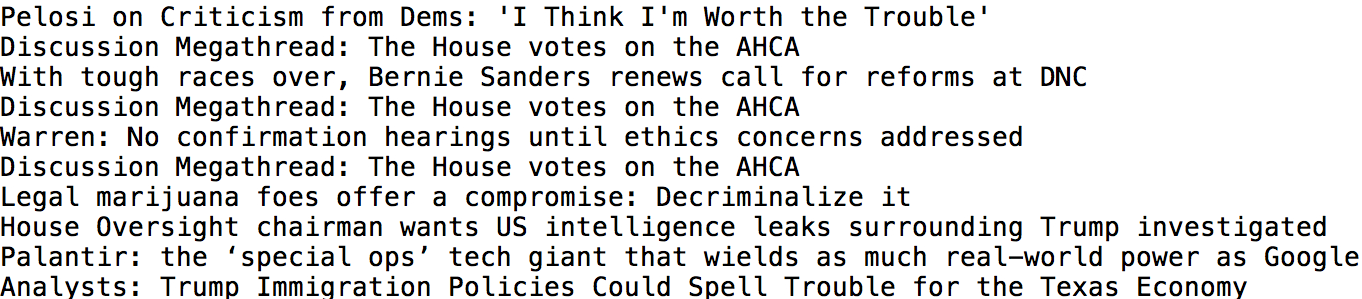
\includegraphics[width=.8\textwidth]{neg10.png}
\end{figure*}
\begin{table}
\begin{tabular}{c}   	
\end{tabular}	
\end{table}
\newpage

\item 2 scatterplots of submission score, comment score v.s. positive, negative comments.
\begin{figure*}[!ht]\centering
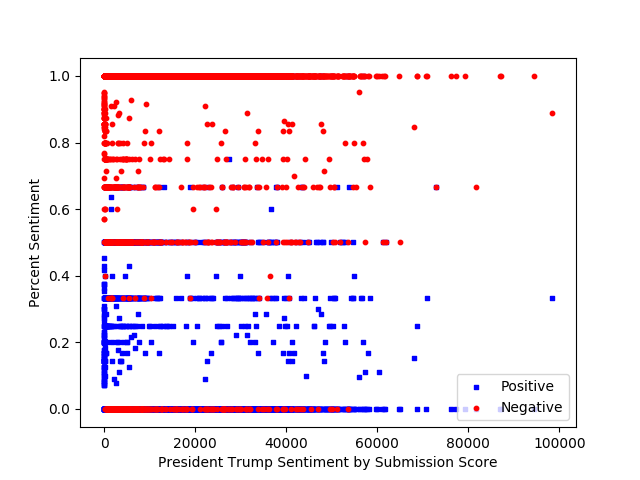
\includegraphics[width=0.7\textwidth]{plot5a.png}\\
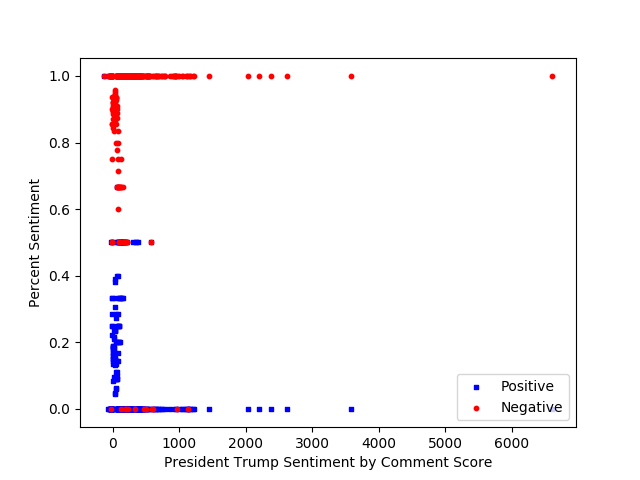
\includegraphics[width=.7\textwidth]{plot5b.png}
\end{figure*}
\newpage
\item NA.
\item NA.
\item Paragraph summarizing the findings.
\begin{itemize}
	\item r/politics mostly has negative comments on President Trump -- over $80\%$ of the comments are negative.
	\item The sentiment certainly varies by state: as shown by the map, with some states in very deep shades and others in light shades. 
	\item Positive or negative sentiments does not seem to vary by time, or at least does not demonstrate a positive trend over time or negative trend over time. But Figure1 demonstrates large variation from day to day -- as both curves are not smooth, and percentage of positive comments have relatively large variance compared to the percentage of negative comments over time.
	\item In terms of comment score, the higher the comment score, the more likely the comment is negative shown by as we move to the right, the red dots are mostly on the  $y$ level of 1.0 and negative dots are on the $y$ level of 0.0. For the comments with less scores, they attract there are are red/blue dots floating round 0.8/0.2, meaning the comments are less polar.
	\item In terms of submission score, the ones with the most upvotes attract a lot of negative comments whereas the submissions with smaller scores, tend to attract more diverse sentiments -- they are not almost exclusively negative.
\end{itemize}
\end{enumerate}
\noindent \textbf{Question 1.} Functional dependencies:\\
\begin{verbatim}
Input_id -> labelgop
Input_id -> labeldem
Input_id -> labeldjt	
\end{verbatim}
\noindent \textbf{Question 2.} The data does not look normalized. The possible redundancies are: 
\begin{itemize}
	\item subreddit name gets repeated for each comment in that subreddit
	\item can\_gild, author\_flair\_text, author\_flair\_css\_classString, author\_cakeday gets repeated for each user whenever he/she posts a comment
\end{itemize}

\noindent Possible decomposition: 
\begin{verbatim}
user_details(userid, can_gild, author_flair_text, author_flair_css_classString, author_cake)
comments(comment_id, user_id, subreddit_id, ... other attributes...)
subreddiit(subreddit_id, name)	
\end{verbatim}
\texttt{comment.user\_id} is a foreign key referencing \texttt{user\_details.user\_id} and \texttt{comments.subreddit\_id} is a foreign key referencing \texttt{subreddit.subreddit\_id}.\\
\noindent The author designed it this way because even though it contains redundancies, the information that we consider redundant may be very relevant in analysis of a comment and if we need to look at these features each time we analyze a comment, obtaining it through joining (with less redundancy) is going to be expensive.\\[1 em]
\newpage
\noindent \textbf{Question 3} Pick one of the joins and run it with \texttt{explain}.\\
\indent We choose to run \texttt{comments.join(labeled\_data, comments.id == labeled\_data.Input\_id).explain()}. The output is the following:
\begin{figure*}[!ht]\centering
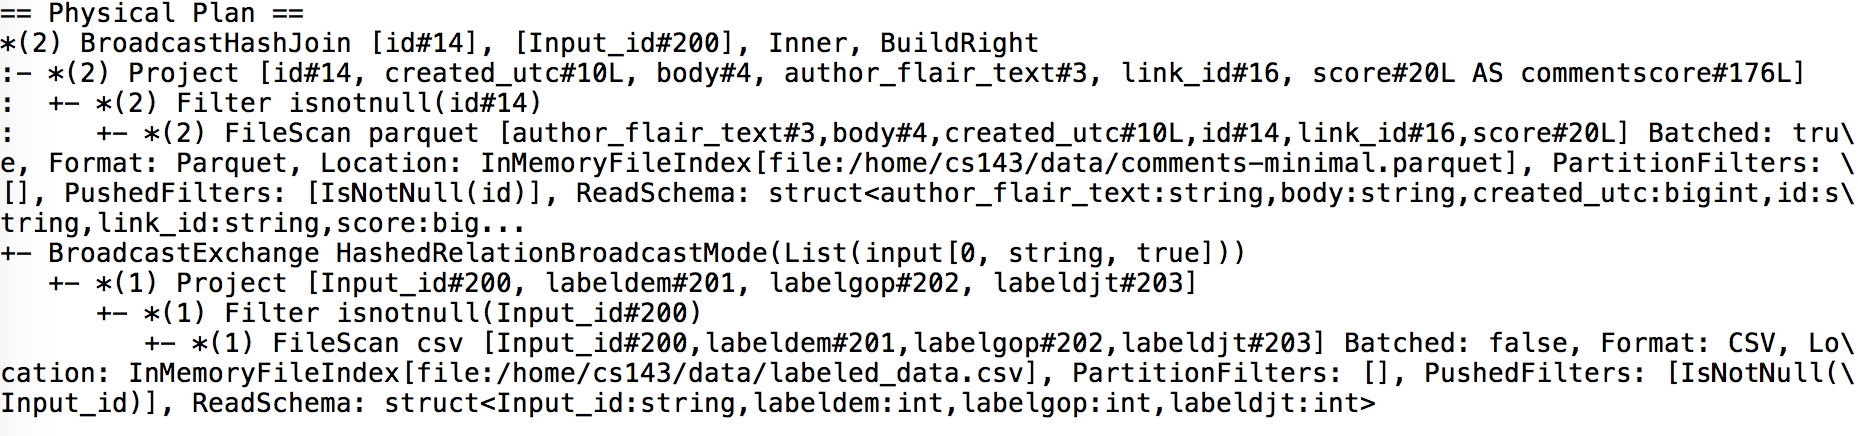
\includegraphics[width=\textwidth]{join_explain.png}	
\end{figure*}

I first noticed that the plan is presented as a tree, the plan executes starting from the leaves (the inner indents) to the root (the top-level indent).

Each node performs a \texttt{FileScan} to read in the data and \texttt{Filter} out the rows where the join key is null, project to the variables that is going to show up into the output. After doing so for each worker, they BoroadcastExchange information so that Spark can better plan and estimate further plan. Finally, it performs the join in the node that handles comments data.

It seems to be using broadcast hash join -- Spark SQL choose to do broadcast hash join when one of the data is smaller than a threshold. In this case, the size of \texttt{labeled\_data.csv}, which is around $30634$ bytes, much smaller than $10$MB, that hinted it to use a \emph{broadcast} hash join. Spark ``broadcasts'' (by having a read-only copy in memory) to every worker node, compared to shipping a copy for each task and it is more efficient in an Spark application where worker nodes communicates through network (since the data gets shipped only once). Among all other types of joins that Spark support (for example, sort-merge join, shuffled hash join, etc), it is the most efficient, however, since we are running this project on a single machine, the performance boost may not be obvious.\texttt{BuildRight} means that the right table -- \texttt{labeled\_data.csv} is the one that is used to create the hash table.
  

\end{document}
